\newpage

\section{Polecenie 8}

Zmiana strategii zapisywania do dziennika rezerwacji. Realizacja przy pomocy triggerów
Należy wprowadzić zmianę która spowoduje że zapis do dziennika rezerwacji będzie realizowany
przy pomocy trigerów

\subsection{TRIGER DODANIE REZERWACJI}
triger obsługujący dodanie rezerwacji

\begin{verbatim}
CREATE OR REPLACE TRIGGER DODANIE_REZERWACJI
  AFTER INSERT
  ON REZERWACJE
  FOR EACH ROW
  DECLARE
    AKTUALNA_DATA DATE;
  BEGIN
    SELECT CURRENT_DATE INTO AKTUALNA_DATA FROM DUAL;
    INSERT INTO DZIENNIK_REZERWACJI (NR_REZERWACJI, DATA, NOWY_STATUS)
    VALUES (:NEW.NR_REZERWACJI, AKTUALNA_DATA, :NEW.STATUS);
  END;
\end{verbatim}

Po dodaniu rezerwacji kodem poniżej:
\begin{verbatim}
begin
  ZMIEN_STATUS_REZERWACJI_3(41, 'Z');
end;
\end{verbatim}

Dziennik rezerwacji:\\
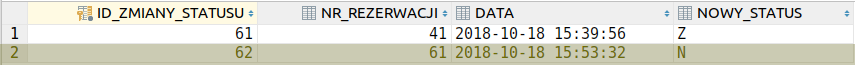
\includegraphics[width=\linewidth]{./images/triger_dodaj_rezerwacje.png}
Rezerwacje:\\
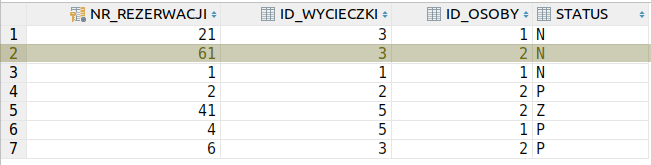
\includegraphics[width=\linewidth]{./images/triger_dodaj_rezerwacje_.png}

\subsection{TRIGER ZMIANA STATUSU}
triger obsługujący zmianę statusu

\begin{verbatim}
CREATE OR REPLACE TRIGGER ZMIANA_STATUSU_REZERWACJI
  AFTER UPDATE
  ON REZERWACJE
  FOR EACH ROW
  DECLARE
    AKTUALNA_DATA DATE;
  BEGIN
    SELECT CURRENT_DATE INTO AKTUALNA_DATA FROM DUAL;
    INSERT INTO DZIENNIK_REZERWACJI (NR_REZERWACJI, DATA, NOWY_STATUS)
    VALUES (:NEW.NR_REZERWACJI, AKTUALNA_DATA, :NEW.STATUS);
  END;
\end{verbatim}

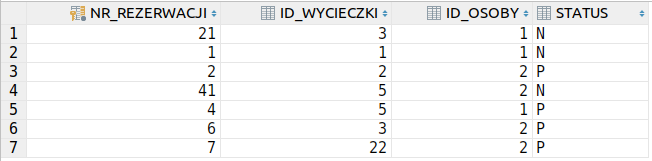
\includegraphics[width=\linewidth]{./images/zmien_status_rezerwacji_3.png}

Po zmianie statusu rezerwacji metodą z sufiksem 3 - przepis podany poniżej.
\begin{verbatim}
begin
  ZMIEN_STATUS_REZERWACJI_3(41, 'Z');
end;
\end{verbatim}

Rezerwacje:\\
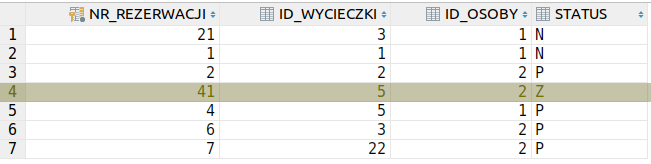
\includegraphics[width=\linewidth]{./images/zmien_status_rezerwacji_3_.png}
Dziennik rezerwacji:\\
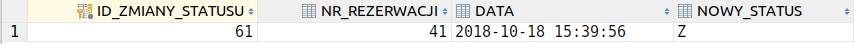
\includegraphics[width=\linewidth]{./images/zmien_status_rezerwacji_3___.png}

\subsection{TRIGER USUWANIE REZERWACJI}
triger zabraniający usunięcia rezerwacji

\subsubsection{TRIGER}
\begin{verbatim}
CREATE OR REPLACE TRIGGER USUWANIE_REZERWACJI
  BEFORE DELETE
  ON REZERWACJE
  BEGIN
    RAISE_APPLICATION_ERROR(-20001, 'RECORDS CAN NOT BE DELETED');
  END;
\end{verbatim}

\subsubsection{POMOCNICZA PROCEDURA}
\begin{verbatim}
CREATE OR REPLACE PROCEDURE USUN_REZERWACJE(ID_R NUMBER)
AS
  BEGIN
    DECLARE
      REZERWACJA NUMBER;
    BEGIN
      SELECT COUNT(R.NR_REZERWACJI) INTO REZERWACJA FROM REZERWACJE R WHERE R.NR_REZERWACJI = ID_R;

      IF REZERWACJA = 1
      THEN
        DELETE FROM REZERWACJE R WHERE R.NR_REZERWACJI = ID_R;
      END IF;
    END;
  END;
\end{verbatim}

Po wykonaniu kodu:
\begin{verbatim}
begin
  USUN_REZERWACJE(6);
end;
\end{verbatim}
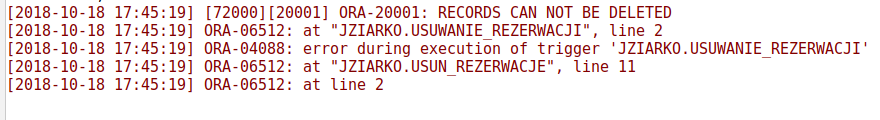
\includegraphics[width=\linewidth]{./images/records_can_not_be_deleted.png}

\subsection{UAKTUALNIONE PROCEDURY MODYFIKUJĄCE DANE}
Oczywiście po wprowadzeniu tej zmiany należy uaktualnić procedury modyfikujące dane.
Najlepiej to zrobić tworząc nowe wersje (np. z sufiksem 3)

\begin{verbatim}
CREATE PROCEDURE ZMIEN_STATUS_REZERWACJI_3(ID_REZERWACJI NUMBER, NOWY_STATUS_ CHAR)
AS
  BEGIN
    DECLARE
      ID_R            NUMBER;
      S               CHAR;
      DZISIEJSZA_DATA DATE;
    BEGIN
      SELECT COUNT(R.NR_REZERWACJI) INTO ID_R FROM REZERWACJE R WHERE R.NR_REZERWACJI = ID_REZERWACJI;
      SELECT R.STATUS INTO S FROM REZERWACJE R WHERE R.NR_REZERWACJI = ID_REZERWACJI;
      SELECT CURRENT_DATE INTO DZISIEJSZA_DATA FROM DUAL;
      IF ID_R = 1
      THEN
        IF (S <> 'A') AND NOWY_STATUS_ IN ('N', 'P', 'Z') AND NOWY_STATUS_ <> S
        THEN
          UPDATE REZERWACJE R SET R.STATUS = NOWY_STATUS_ WHERE R.NR_REZERWACJI = ID_REZERWACJI;
        END IF;
      END IF;
    END;
  END;
\end{verbatim}
 